\section{Results}
\label{sec:results}

This section presents the main results of the FRESNEL field campaign,
focusing on the integration of model forecasts, target sampling, and
data assimilation using autonomous underwater vehicles (AUVs). The
analysis combines CMS and statistical model forecasts (as described
in the Methods section) with in situ observations to assess how the
proposed data-cycle approach can enhance short-term ocean prediction
in a dynamic coastal environment.

Fig. \ref{fig:sst} provides an overview of the environmental conditions
observed during the three-day experimental window considered in this
study (29–31 October). The background fields correspond to the Level-3
Sea Surface Temperature (SST) product from Copernicus Marine Service
(\url{DOI:10.48670/moi-00310}). The operational area was relatively
compact, covering approximately 100 km² south of the Nazaré Canyon,
where the AUVs executed the planned target sampling missions. All
missions were planned using the target sampling algorithm to explore the
temperature variability predicted by the statistical model. On 31
October, however, XP2 performed a different mission, following a
cross-shore transect of approximately 13 km instead of a target-driven
pattern north of the canyon. This mission was designed to sample an
internal wave hotspot, but, for the purpose of this study, it serves as
an independent ground-truth dataset, collected in a distinct subregion
relative to where the data assimilation was applied. The XP2
observations are thus used as a reference for evaluating the forecast
cases (C–C4 and D–D4).

During this period, the coastal ocean was influenced by a late-season
upwelling–relaxation cycle. At the beginning of the sequence (29
October), the SST field reveals the characteristic signature of coastal
upwelling, with colder water masses extending offshore due to
wind-driven Ekman transport that brings subsurface, nutrient-rich waters
to the surface. In the following days (30–31 October), the weakening of
upwelling-favorable winds led to a relaxation phase, during which warmer
offshore waters gradually advanced toward the coast. This transition is
reflected in the SST maps by an overall warming trend in the nearshore
region, particularly evident on 1st October.

It is important to note that the SST imagery is partially affected by
cloud coverage, which limits the availability and accuracy of
satellite-derived temperature data. These gaps arise from the
radiometric constraints of indirect SST retrieval, resulting in reduced
spatial continuity and increased uncertainty near cloudy regions.
Despite these limitations, the SST patterns clearly capture the dominant
mesoscale features and coastal processes driving the observed
variability during the experiment.

These evolving conditions provided an ideal natural setting for testing
the adaptive sampling and data assimilation framework developed in
FRESNEL. The pronounced temperature gradients associated with the
upwelling front generated well-defined spatial and temporal variability,
allowing the evaluation of how AUV-based targeted observations can
improve the predictive skill of the statistical model in a real-world
coastal scenario.

Following the overview of the surface conditions,
Fig.\ref{fig:temperatureprofiles} presents the vertical temperature
distribution recorded by the LAUVs XP2, XP3, and XP5 during their
respective missions between 29 and 31 October. The panels show
temperature as a function of time and depth, illustrating the temporal
and vertical structure of the coastal water column throughout the
three-day experimental sequence.

XP2 operated on 29 October, XP5 on 29, 30, and 31 October, and XP3 on 30
and 31 October, with all vehicles capable of sampling the upper 100 m of
the water column. However, this depth range was not always achieved due
to logistical and bathymetric constraints. The temperature fields reveal
a thermocline and a progressive warming of the surface layer down to
approximately 40 m depth, with temperatures ranging from around 14 °C in
deeper layers to about 18 °C near the surface, reaching their maximum on
30 October afternoon during XP5’s mission.

It is important to note that the trajectories shown in the previous
figure might suggest that the AUVs remained continuously at sea for 24
hours each day. However, as Fig. \ref{fig:temperatureprofiles}
demonstrates, this was not the case. The vehicles can be deployed and
recovered multiple times per day, with operational windows limited by
logistics, weather, and available support assets. This figure,
therefore, also highlights the non-linear nature of field logistics in
multi-vehicle operations, where dynamic scheduling, resource allocation,
and environmental constraints determine the actual temporal coverage of
the missions.

\begin{figure}
  \centering 

  \subfigure[Sea surface temperature (SST) and XP2, XP3 and
  XP5 trajectories during the FRESNEL field campaign (29–31
  October).]{\label{fig:sst}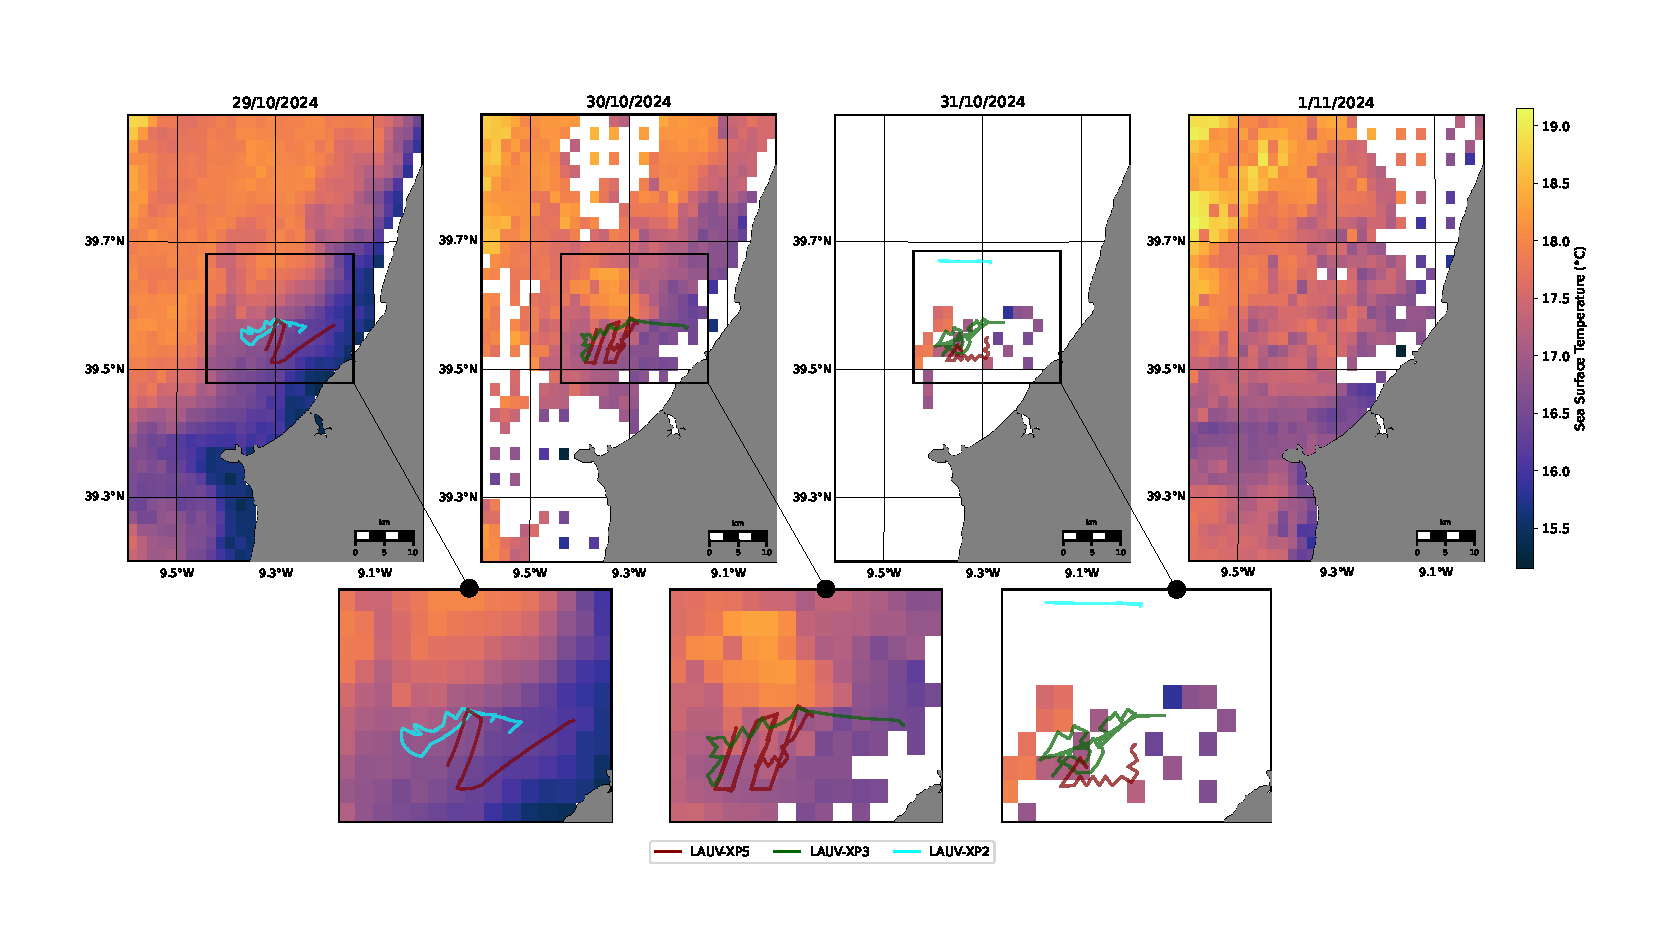
\includegraphics[width=1\linewidth]{fig/Figure_sst_auv_l3_zoom.pdf}}

  \subfigure[Time–depth temperature evolution observed by XP2, XP3, and
  XP5 during the FRESNEL field campaign (29–31
  October).]{\label{fig:temperatureprofiles}\includegraphics[width=1\linewidth]{fig/Figure2_100m.pdf}}

\end{figure}




\begin{itemize}
    \item Environmental context
    
    \item RMS table (all cases) + rms figure (just A+D cases)
\end{itemize}

 
\textit{- Use \textbf{subheadings} to organize different experiments or analyses.}
